% Tento soubor nahraďte vlastním souborem s přílohami (nadpisy níže jsou pouze pro příklad)
% This file should be replaced with your file with an appendices (headings below are examples only)

% Umístění obsahu paměťového média do příloh je vhodné konzultovat s vedoucím
% Placing of table of contents of the memory media here should be consulted with a supervisor
%\chapter{Obsah přiloženého paměťového média}

\chapter{CD Content}
\label{CD Content}

\begin{itemize}
  \item \textbf{/maestro-java/*}\,---\,source code of Maestro from date \today
  \item \textbf{/iqa-topology-generator/*}\,---\,source code of Topology Generator from date \today
  \item \textbf{/doc/*}\,---\,Maestro documentation
  \item \textbf{/readme.txt}\,---\,readme with useful informations about Maestro build and start
  \item \textbf{/text/*}\,---\,source code of this thesis from date \today
  \item \textbf{/xstejs24-performance.pdf}\,---\,final version of this thesis from date \today
\end{itemize}

\chapter{The Maestro Protocol}
\label{AP:commands}
The following commands were updated according the Maestro 1.3.0 version\footnote{Original commands description for MPT is available at \url{https://github.com/orpiske/msg-perf-tool/tree/master/doc/maestro/protocol}}:

\section*{Requests Notes}
\begin{description}
  \setlength\itemsep{0em}
  \item \textbf{MAESTRO\_NOTE\_START\_RECEIVER}\,---\,note to the receiver, that it should start receiving data.
  \begin{itemize}
    \setlength\itemsep{0em}
    \item Value: 0
    \item Payload: None
    \item Response: the peers respond to this note by sending a MAESTRO\_NOTE\_OK or MAESTRO\_NOTE\_INTERNAL\_ERROR
  \end{itemize}
  \item \textbf{MAESTRO\_NOTE\_STOP\_RECEIVER}\,---\,note to the receiver, that it should stop receiving data.
  \begin{itemize}
    \setlength\itemsep{0em}
    \item Value: 1
    \item Payload: None
    \item Response: the peers respond to this note by sending a MAESTRO\_NOTE\_OK or MAESTRO\_NOTE\_INTERNAL\_ERROR
  \end{itemize}
  \item \textbf{MAESTRO\_NOTE\_START\_SENDER}\,---\,note to the sender, that it should start sending data.
  \begin{itemize}
    \setlength\itemsep{0em}
    \item Value: 2
    \item Payload: None
    \item Response: the peers respond to this note by sending a MAESTRO\_NOTE\_OK or MAESTRO\_NOTE\_INTERNAL\_ERROR
  \end{itemize}
  \item \textbf{MAESTRO\_NOTE\_STOP\_SENDER}\,---\,note to the sender, that it should stop sending data.
  \begin{itemize}
    \setlength\itemsep{0em}
    \item Value: 3
    \item Payload: None
    \item Response: the peers respond to this note by sending a MAESTRO\_NOTE\_OK or MAESTRO\_NOTE\_INTERNAL\_ERROR
  \end{itemize}
  \item \textbf{MAESTRO\_NOTE\_START\_INSPECTOR}\,---\,note to the inspector, that it should start inspecting the SUT.
  \begin{itemize}
    \setlength\itemsep{0em}
    \item Value: 4
    \item Payload: None
    \item Response: the peers respond to this note by sending a MAESTRO\_NOTE\_OK or MAESTRO\_NOTE\_INTERNAL\_ERROR
  \end{itemize}
  \item \textbf{MAESTRO\_NOTE\_STOP\_INSPECTOR}\,---\,note to the inspector, that it should stop inspecting the SUT.
  \begin{itemize}
    \setlength\itemsep{0em}
    \item Value: 5
    \item Payload: None
    \item Response: the peers respond to this note by sending a MAESTRO\_NOTE\_OK or MAESTRO\_NOTE\_INTERNAL\_ERROR
  \end{itemize}
  \item \textbf{MAESTRO\_NOTE\_FLUSH}\,---\,note to the any node to request it to flush test data to disk.
  \begin{itemize}
    \setlength\itemsep{0em}
    \item Value: 6
    \item Payload: None
    \item Response: the peers respond to this note by sending a MAESTRO\_NOTE\_OK or MAESTRO\_NOTE\_INTERNAL\_ERROR
  \end{itemize}
  \item \textbf{MAESTRO\_NOTE\_SET}\,---\,note to the any node to set the testing properties.
  \begin{itemize}
    \setlength\itemsep{0em}
    \item Value: 7
    \item Payload: the test parameters such as TEST\_DURATION, PARALLEL\_COUNT, MESSAGE\_SIZE, RATE, etc.
    \item Response: the peers respond to this note by sending a MAESTRO\_NOTE\_OK or MAESTRO\_NOTE\_INTERNAL\_ERROR
  \end{itemize}
  \item \textbf{MAESTRO\_NOTE\_STATS}\,---\,note to the any node to request the current performance statistics.
  \begin{itemize}
    \setlength\itemsep{0em}
    \item Value: 8
    \item Payload: None
    \item Response: the peers respond to this note by sending a MAESTRO\_NOTE\_OK or MAESTRO\_NOTE\_INTERNAL\_ERROR
  \end{itemize}
  \item \textbf{MAESTRO\_NOTE\_HALT}\,---\,note to the any node to request them to stop and exit cleanly.
  \begin{itemize}
    \setlength\itemsep{0em}
    \item Value: 9
    \item Payload: None
    \item Response: the peers respond to this note by sending a MAESTRO\_NOTE\_OK or MAESTRO\_NOTE\_INTERNAL\_ERROR
  \end{itemize}
  \item \textbf{MAESTRO\_NOTE\_PING}\,---\,note to the any node to verify which peers are alive in the cluster.
  \begin{itemize}
    \setlength\itemsep{0em}
    \item Value: 10
    \item Payload: seconds or microseconds.
    \item Response: the peers respond to this note by sending a MAESTRO\_NOTE\_OK or MAESTRO\_NOTE\_INTERNAL\_ERROR
  \end{itemize}
  \item \textbf{MAESTRO\_NOTE\_GET}\,---\,note to the peers to get informations about the test.
  \begin{itemize}
    \setlength\itemsep{0em}
    \item Value: 17
    \item Payload: None
    \item Response:
  \end{itemize}
  \item \textbf{MAESTRO\_NOTE\_START\_AGENT}\,---\,note to the agent, that it should start executing external handlers.
  \begin{itemize}
    \setlength\itemsep{0em}
    \item Value: 18
    \item Payload: None
    \item Response: the peers respond to this note by sending a MAESTRO\_NOTE\_OK or MAESTRO\_NOTE\_INTERNAL\_ERROR
  \end{itemize}
  \item \textbf{MAESTRO\_NOTE\_STOP\_AGENT}\,---\,note to the agent, that it should stop executing external handlers.
  \begin{itemize}
    \setlength\itemsep{0em}
    \item Value: 19
    \item Payload: None
    \item Response: the peers respond to this note by sending a MAESTRO\_NOTE\_OK or MAESTRO\_NOTE\_INTERNAL\_ERROR
  \end{itemize}
  \item \textbf{MAESTRO\_NOTE\_AGENT\_SOURCE}\,---\,note to the agent, that it should download external source defined in the payload.
  \begin{itemize}
    \setlength\itemsep{0em}
    \item Value: 21
    \item Payload: URL for external git repository which the Agent will download.
    \item Response: the peers respond to this note by sending a MAESTRO\_NOTE\_OK or MAESTRO\_NOTE\_INTERNAL\_ERROR
  \end{itemize}
  \item \textbf{MAESTRO\_NOTE\_USER\_COMMAND\_1}\,---\,note to the agent, that it should execute command specified in the payload. The command should be present in external git repository downloaded by MAESTRO\_NOTE\_AGENT\_SOURCE.
  \begin{itemize}
    \setlength\itemsep{0em}
    \item Value: 30
    \item Payload: Command which will be executed in string format.
    \item Response: the peers respond to this note by sending a MAESTRO\_NOTE\_OK or MAESTRO\_NOTE\_INTERNAL\_ERROR
  \end{itemize}
\end{description}


\section*{Response Notes}
\begin{description}
  \setlength\itemsep{0em}
  \item \textbf{MAESTRO\_NOTE\_STATS}\,---\,is sent by a node as a response to a MAESTRO\_NOTE\_STATS request.
  \begin{itemize}
    \setlength\itemsep{0em}
    \item Value: 8
    \item Payload: yes
  \end{itemize}
  \item \textbf{MAESTRO\_NOTE\_PING}\,---\,is sent by the peers as a response to a MAESTRO\_NOTE\_PING request.
  \begin{itemize}
    \setlength\itemsep{0em}
    \item Value: 10
    \item Payload: yes
  \end{itemize}
  \item \textbf{MAESTRO\_NOTE\_OK}\,---\,is a generic response when the node complies with a request.
  \begin{itemize}
    \setlength\itemsep{0em}
    \item Value: 11
    \item Payload: None
  \end{itemize}
  \item \textbf{MAESTRO\_NOTE\_PROTOCOL\_ERROR}\,---\,is issued by any node whenever the protocol is malformed.
  \begin{itemize}
    \setlength\itemsep{0em}
    \item Value: 12
    \item Payload: None
  \end{itemize}
  \item \textbf{MAESTRO\_NOTE\_INTERNAL\_ERROR}\,---\,is issued by any node when it is unable to comply with a request.
  \begin{itemize}
    \setlength\itemsep{0em}
    \item Value: 13
    \item Payload: None
  \end{itemize}
  \item \textbf{MAESTRO\_NOTE\_ABNORMAL\_DISCONNECT}\,---\,is issued by any node as a last-will message.
  \begin{itemize}
    \setlength\itemsep{0em}
    \item Value: 14
    \item Payload: None
  \end{itemize}
\end{description}


\section*{Notify Notes}
\begin{description}
  \setlength\itemsep{0em}
  \item \textbf{MAESTRO\_NOTE\_NOTIFY\_FAIL}\,---\,is issued by any node when the test failed.
  \begin{itemize}
    \setlength\itemsep{0em}
    \item Value: 15
    \item Payload: yes
  \end{itemize}
  \item \textbf{MAESTRO\_NOTE\_NOTIFY\_SUCCESS}\,---\,is issued by any node when the test completed successfully.
  \begin{itemize}
    \setlength\itemsep{0em}
    \item Value: 16
    \item Payload: yes
  \end{itemize}
\end{description}


\chapter{Topology Generator} % Configuration filenechce

\section*{Inventory}
\label{AP:Inventory}
The following is an example of Inventory file used as an input for Topology Generator and Ansible deployment scripts. The inventory lists all the nodes and their role in the topology.

\begin{verbatim}
[clients]
sender ansible_host=10.0.0.1
receiver ansible_host=10.0.0.2

[routers]
router1 ansible_host=10.0.0.3
router2 ansible_host=10.0.0.4

[brokers]
broker1 ansible_host=10.0.0.5

[nodes:children]
brokers
clients
routers
\end{verbatim}

\section*{Graph Metadata}
\label{AP:Graph Metadata}
The example of graph metadata file for Topology Generator is as follows. For this case Generator will generate graph with two routers and three brokers, where routers are connected together and each broker is connected to one router.

\begin{verbatim}
---
directed: false
graph: {}
nodes:
- type: router						%node type
  id: router1						%node name
- type: router
  id: router2
- type: broker
  id: broker1
- type: broker
  id: broker2
links:
- source: router2					%source node for link
  target: router1					%target node for link
- source: router2
  target: broker2
- source: router1
  target: broker1
multigraph: false
\end{verbatim}

\section*{Topology Generator Output}
\label{AP:Topology Generator Output}
The example of Topology Generator output in YAML format. This output is for two directly connected routers.

\begin{verbatim}
---
confs:
- machine: router1
  router:
  - id: router1
    mode: standalone
  listener:
  - host: 0.0.0.0
    role: inter-router
    port: 6000
  - host: 0.0.0.0
    authenticatePeer: 'no'
    role: normal
    port: 5000
    saslMechanisms: ANONYMOUS
  connector:
  - host: router2
    role: inter-router
    port: 6001
  address:
  - prefix: closest
    distribution: closest
  - prefix: multicast
    distribution: multicast
  - prefix: unicast
    distribution: closest
- machine: router2
  router:
  - id: router2
    mode: standalone
  listener:
  - host: 0.0.0.0
    role: inter-router
    port: 6001
  - host: 0.0.0.0
    authenticatePeer: 'no'
    role: normal
    port: 5001
    saslMechanisms: ANONYMOUS
  connector:
  - host: router1
    role: inter-router
    port: 6000
  address:
  - prefix: closest
    distribution: closest
  - prefix: multicast
    distribution: multicast
  - prefix: unicast
    distribution: closest

\end{verbatim}

\section*{Qpid-Dispatch Configuration File Template}
\label{AP:Qpid-Dispatch Configuration File Template}
The template for configuration files for current version of Qpid-Dispatch is generated by \emph{qdrouter-jinja2} tool which is open-source and available at \url{https://github.com/rh-messaging-qe/qdrouter-jinja2}.

Since the template is file with approximately 600 lines, the model template for Qpid-Dispatch version 1.0.0 is available at \url{https://github.com/rh-messaging-qe/ansible-qpid-dispatch/blob/master/test/files/templates/qdrouterd-roland.conf.j2}.

\section*{Topology Generator Source Code}
\label{AP:Topology Generator Source Code}
The complete source code of Topology Generator is available at:
\begin{itemize}
  \item \url{https://github.com/rh-messaging-qe/iqa-topology-generator}
  \item \url{https://pypi.org/project/msg-topgen/#description}
\end{itemize}


\chapter{AMQP Inspector Data Sets}
\label{AMQP Inspector Data Sets}
The following represents headers for data files with AMQP Inspector collected data. The data file structure depends on the AMQP Inspector request.

\section*{General Info}
\begin{itemize}
  \setlength\itemsep{0em}
  \item \textbf{Timestamp}\,---\,timestamp when the data was collected.
  \item \textbf{Name}\,---\,name of the router.
  \item \textbf{Version}\,---\,version of the router.
  \item \textbf{LinkRoutes}\,---\,number of active link routes.
  \item \textbf{AutoLinks}\,---\,number of active auto links.
  \item \textbf{Links}\,---\,number of active links.
  \item \textbf{Nodes}\,---\,number of active neighbour nodes.
  \item \textbf{Addresses}\,---\,number of active addresses.
  \item \textbf{Connections}\,---\,number of active connections.
\end{itemize}

\section*{Memory Info}
\begin{itemize}
  \setlength\itemsep{0em}
  \item \textbf{Timestamp}\,---\,timestamp when the data was collected.
  \item \textbf{Name}\,---\,name of the memory space.
  \item \textbf{Size}\,---\,type size.
  \item \textbf{Batch}\,---\,transfer batch size.
  \item \textbf{Thread-max}\,---\,maximum allocated for thread.
  \item \textbf{Total}\,---\,totally allocated memory.
  \item \textbf{In-threads}\,---\,memory held by threads.
  \item \textbf{Rebal-in}\,---\,batches rebalanced to threads.
  \item \textbf{Rebal-out}\,---\,batches rebalanced to global.
  \item \textbf{totalFreeToHeap}\,---\,total free to heap.
  \item \textbf{globalFreeListMax}\,---\,global free list max.
\end{itemize}


\section*{RouteLink Info}
\begin{itemize}
  \setlength\itemsep{0em}
  \item \textbf{Timestamp}\,---\,timestamp when the data was collected.
  \item \textbf{Name}\,---\,name of the route link.
  \item \textbf{LinkDir}\,---\,intput link or output link.
  \item \textbf{OperStatus}\,---\,current status.
  \item \textbf{Identity}\,---\,identification.
  \item \textbf{DeliveryCount}\,---\,number of delivered messages.
  \item \textbf{UndeliveredCount}\,---\,number of undelivered messages.
  \item \textbf{PresettledCount}\,---\,number of presettled messages.
  \item \textbf{UnsettledCount}\,---\,number of unsettled messages.
  \item \textbf{ReleasedCount}\,---\,number of released messages.
  \item \textbf{ModifiedCount}\,---\,number of modified messages.
  \item \textbf{AcceptedCount}\,---\,number of accepted messages.
  \item \textbf{RejectedCount}\,---\,number of rejected messages.
  \item \textbf{Capacity}\,---\,route link capacity.
\end{itemize}

\chapter{Experimental Evaluation Additional Data}
\label{Experimental Evaluation Additional Data}

\section*{Throughput}
The Qpid-Dispatch need some time to evaluate the messages and send them to the receiver. In the Figure \ref{fig:router-single-routerLink} we can see the histogram of unsettled messages during the singlepoint throughput test. This charts shows the number off received messages, which are not yet evaluated. Note, that throughput is around 90,000 messages per second.

The flow-control mechanism mentioned in the Subsection \ref{Throughput} also affected the unsettled message count, which is multiple times higher than in the previous test case depicted in the Figure \ref{fig:router-single-routerLink}. The unsettled message count is depicted in the Figure \ref{fig:router-multipoint-routerLink}.

\begin{figure}[H]
	\centering
	\begin{minipage}{0.49\linewidth}
		\subfloat[Single router node.\label{fig:router-single-routerLink}]{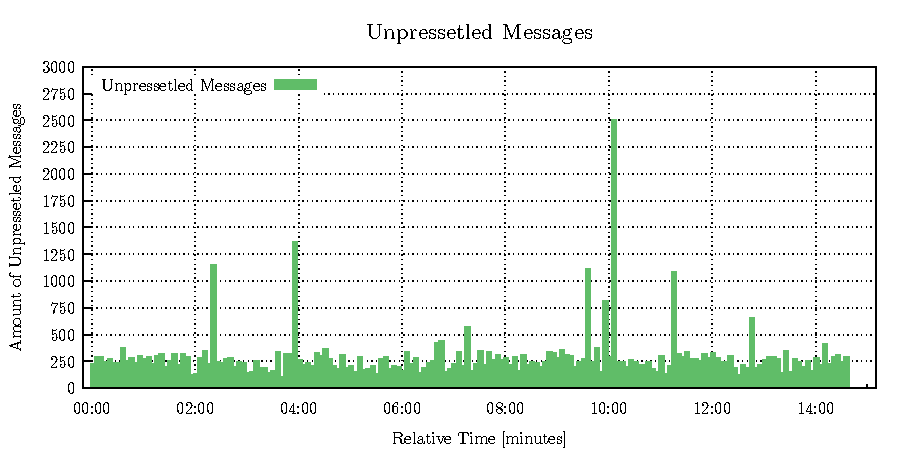
\includegraphics[width=\linewidth]{obrazky-figures/charts/singlepoint-router-throughput-routerLink.pdf}}
	\end{minipage}
	\begin{minipage}{0.49\linewidth}
		\subfloat[Line topology node.\label{fig:router-multipoint-routerLink}]{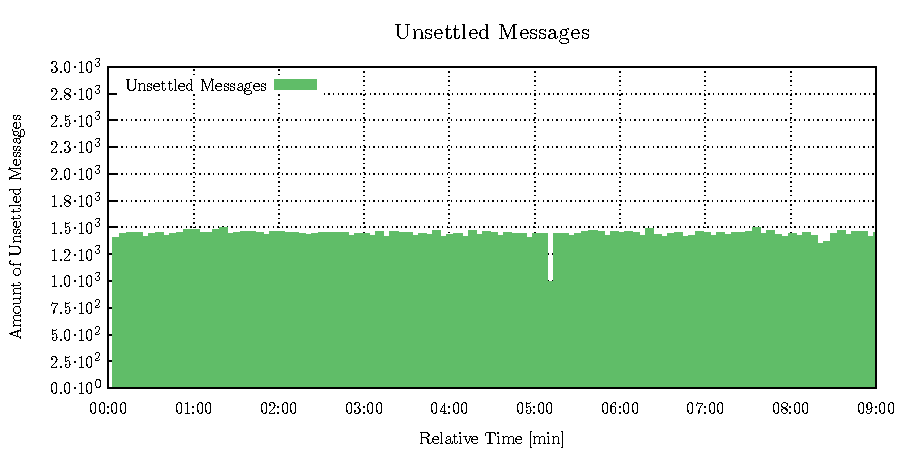
\includegraphics[width=\linewidth]{obrazky-figures/charts/multipoint-router-only-throughput-routerLink.pdf}}
	\end{minipage}
	\caption[Examples of experimental topologies created for basic performance testing and experiments with Maestro.]{Examples of experimental topologies created for basic performance testing and experiments with Maestro.}
  \label{fig:routerLink-throughput}
\end{figure}

\section*{Latency}

Unsettled messages for the router available in the Figure \ref{fig:latency-router-routerLink}. From the Inspector outputs one can see, that the Broker handled 10,000,000 messages in more than 7\,minutes, but the router handled the same amount of messages much faster approximately in 2\,minutes and 20\,seconds.

Since the router applies the flow control during this measurement and the rate is setup to 80\,\% of maximum, the unsettled message count is here much lower than in the other cases as it is depicted in the Figure \ref{fig:latency-multiple-router-routerLink}.

\begin{figure}[H]
	\centering
	\begin{minipage}{0.49\linewidth}
		\subfloat[Single router node.\label{fig:latency-router-routerLink}]{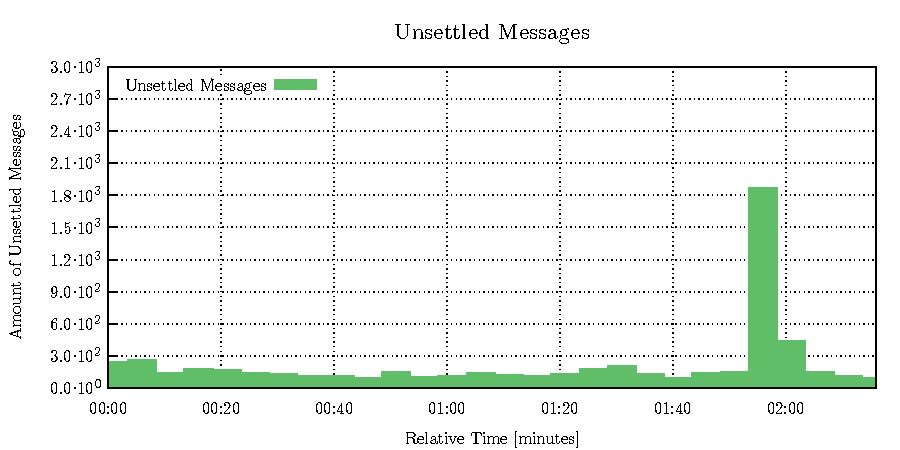
\includegraphics[width=\linewidth]{obrazky-figures/charts/singlepoint-router-latency-routerLink.pdf}}
	\end{minipage}
	\begin{minipage}{0.49\linewidth}
		\subfloat[Line topology node.\label{fig:latency-multiple-router-routerLink}]{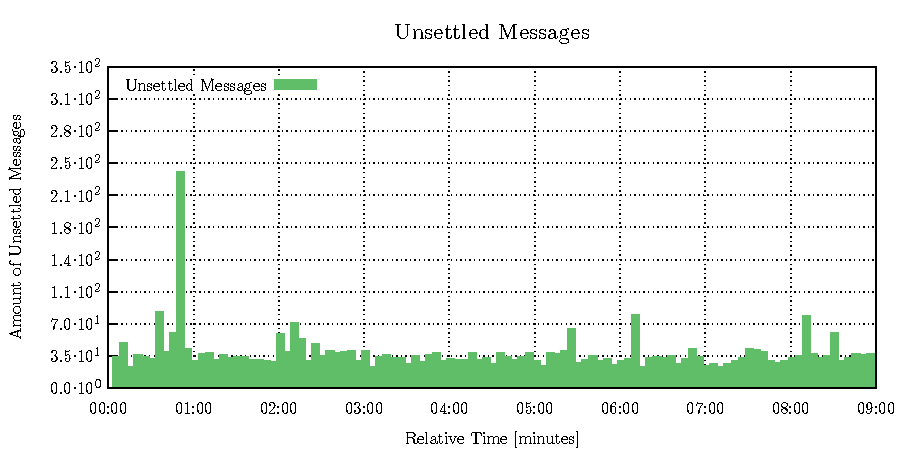
\includegraphics[width=\linewidth]{obrazky-figures/charts/multipoint-router-only-latency-routerLink.pdf}}
	\end{minipage}
	\caption[Examples of experimental topologies created for basic performance testing and experiments with Maestro.]{Examples of experimental topologies created for basic performance testing and experiments with Maestro.}\label{fig:routerLink-latency}
\end{figure}

\section*{Measurement With Redundant Router}

\begin{figure}[h]
	\centering
	\begin{minipage}{0.49\linewidth}
		\subfloat[Restart\label{fig:restart-redundant-agent-memory}]{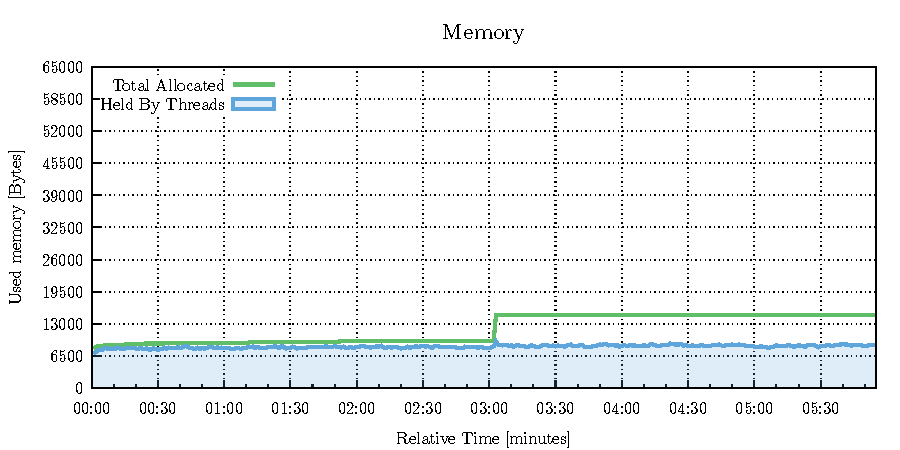
\includegraphics[width=\linewidth]{obrazky-figures/charts/restart-redundant-agent-memory.pdf}}
	\end{minipage}
	\begin{minipage}{0.49\linewidth}
		\subfloat[10 seconds shutdown\label{fig:shutdown_10-redundant-agent-memory}]{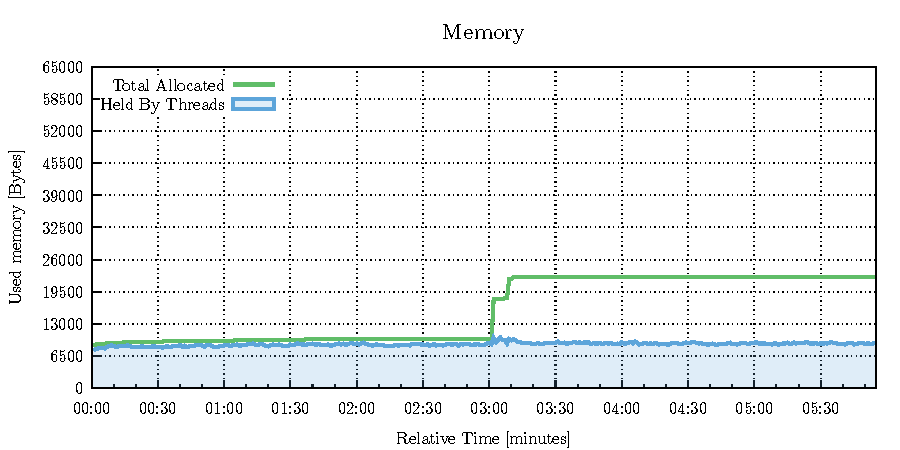
\includegraphics[width=\linewidth]{obrazky-figures/charts/shutdown_10-redundant-agent-memory.pdf}}
	\end{minipage}
  \begin{minipage}{0.49\linewidth}
		\subfloat[60 seconds shutdown\label{fig:shutdown_60-redundant-agent-memory}]{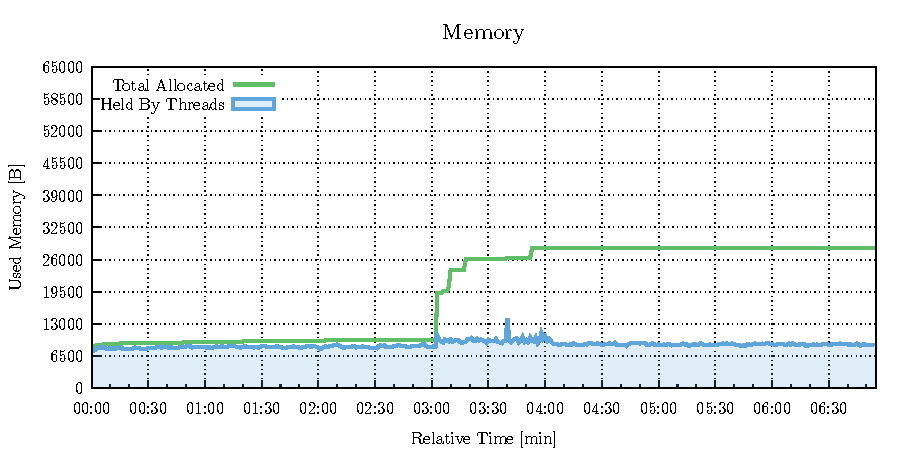
\includegraphics[width=\linewidth]{obrazky-figures/charts/shutdown_60-redundant-agent-memory.pdf}}
	\end{minipage}
	\begin{minipage}{0.49\linewidth}
		\subfloat[120 seconds shutdown\label{fig:shutdown_120-redundant-agent-memory}]{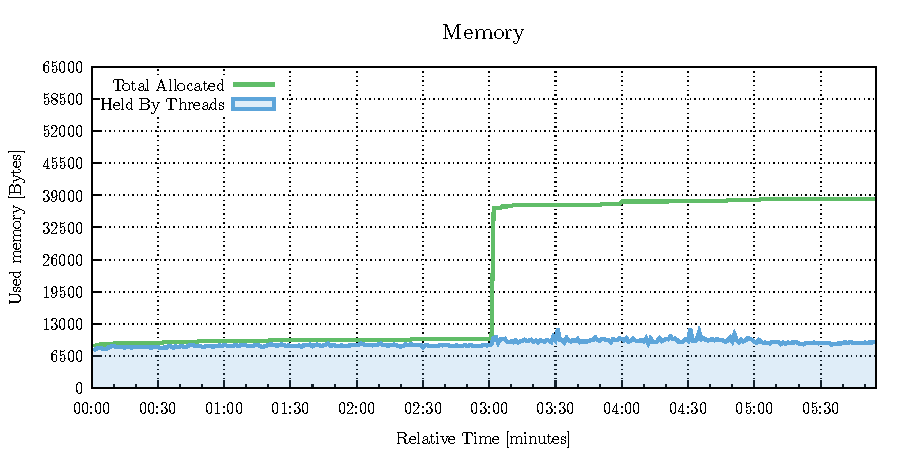
\includegraphics[width=\linewidth]{obrazky-figures/charts/shutdown_120-redundant-agent-memory.pdf}}
	\end{minipage}
	\caption[Collected data about the memory allocation for the redundant router node during the Agent actions execution.]{Collected data about the memory allocation for the redundant router node during the Agent actions execution.}\label{fig:redundant-memory-info}
\end{figure}

\begin{figure}[h]
	\centering
	\begin{minipage}{0.49\linewidth}
		\subfloat[Restart\label{fig:restart-redundant-agent-routerLink}]{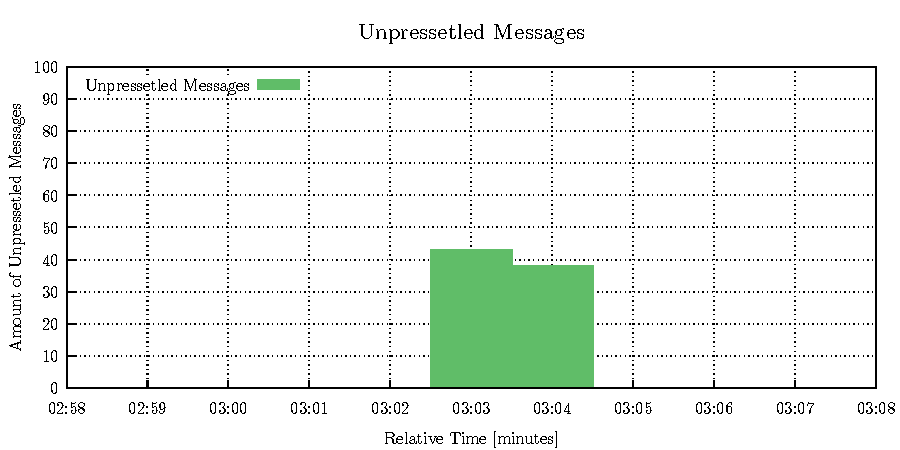
\includegraphics[width=\linewidth]{obrazky-figures/charts/restart-redundant-agent-routerLink.pdf}}
	\end{minipage}
	\begin{minipage}{0.49\linewidth}
		\subfloat[10 seconds shutdown\label{fig:shutdown_10-redundant-agent-routerLink}]{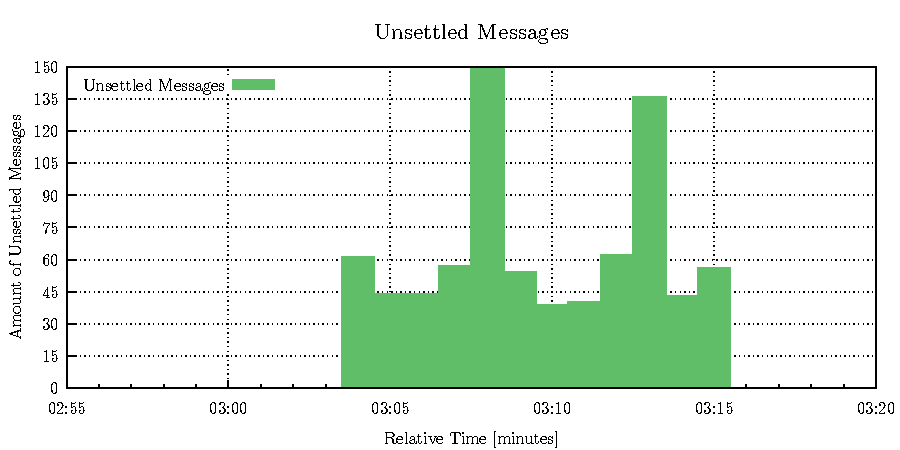
\includegraphics[width=\linewidth]{obrazky-figures/charts/shutdown_10-redundant-agent-routerLink.pdf}}
	\end{minipage}
  \begin{minipage}{0.49\linewidth}
		\subfloat[60 seconds shutdown\label{fig:shutdown_60-redundant-agent-routerLink}]{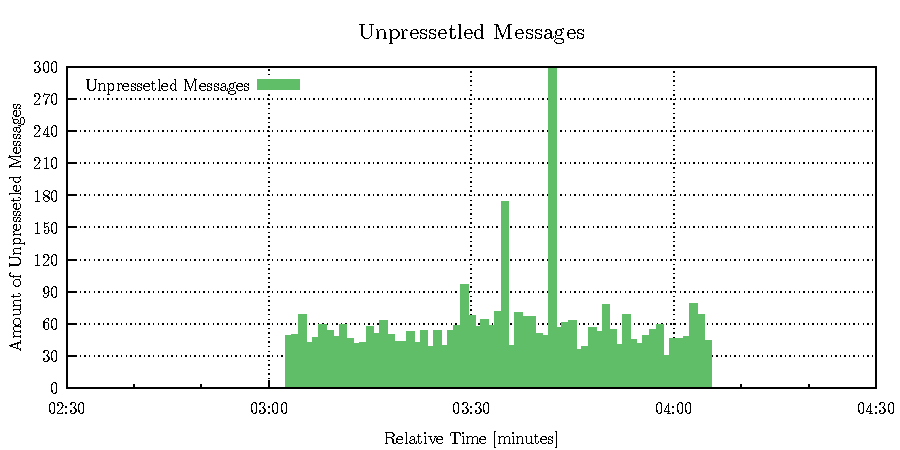
\includegraphics[width=\linewidth]{obrazky-figures/charts/shutdown_60-redundant-agent-routerLink.pdf}}
	\end{minipage}
	\begin{minipage}{0.49\linewidth}
		\subfloat[120 seconds shutdown\label{fig:shutdown_120-redundant-agent-routerLink}]{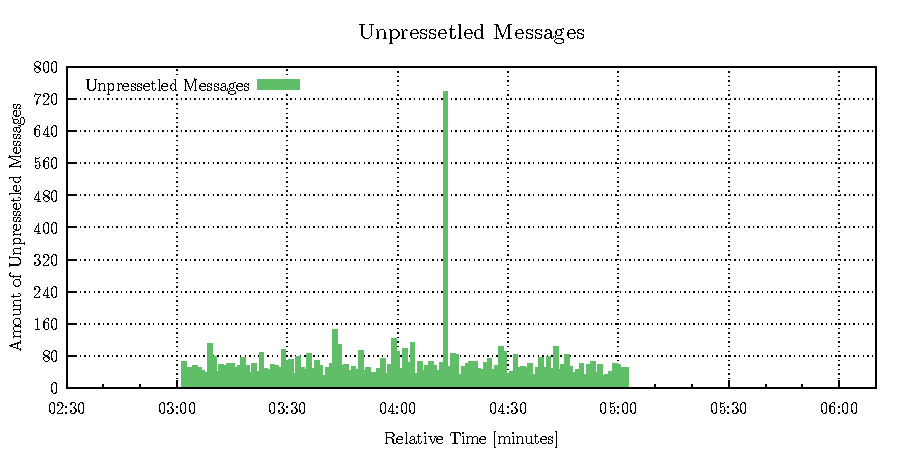
\includegraphics[width=\linewidth]{obrazky-figures/charts/shutdown_120-redundant-agent-routerLink.pdf}}
	\end{minipage}
	\caption[Collected data about the unsettled messages for the redundant router node during the Agent actions execution.]{Collected data about the unsettled messages for the redundant router node during the Agent actions execution.}\label{fig:routerLink-latency}
\end{figure}

\begin{figure}[h]
	\centering
	\begin{minipage}{0.49\linewidth}
		\subfloat[Restart\label{fig:restart-redundant-agent-delivered}]{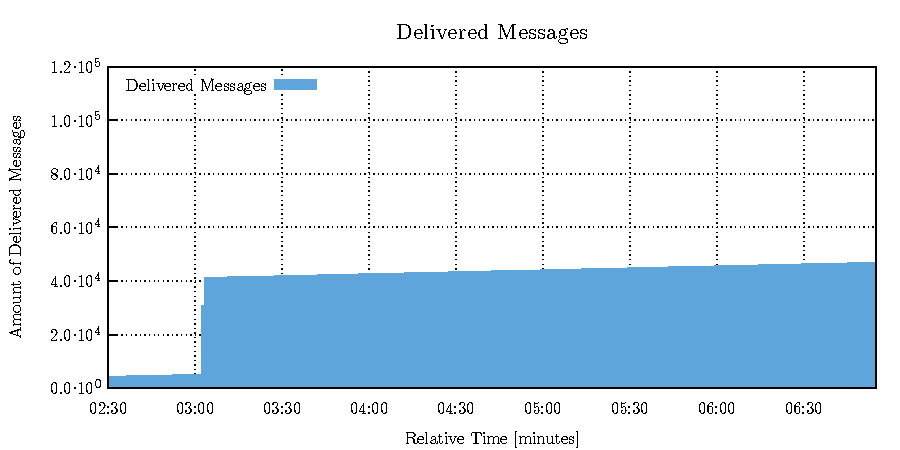
\includegraphics[width=\linewidth]{obrazky-figures/charts/restart-redundant-agent-delivered.pdf}}
	\end{minipage}
	\begin{minipage}{0.49\linewidth}
		\subfloat[10 seconds shutdown\label{fig:shutdown_10-redundant-agent-delivered}]{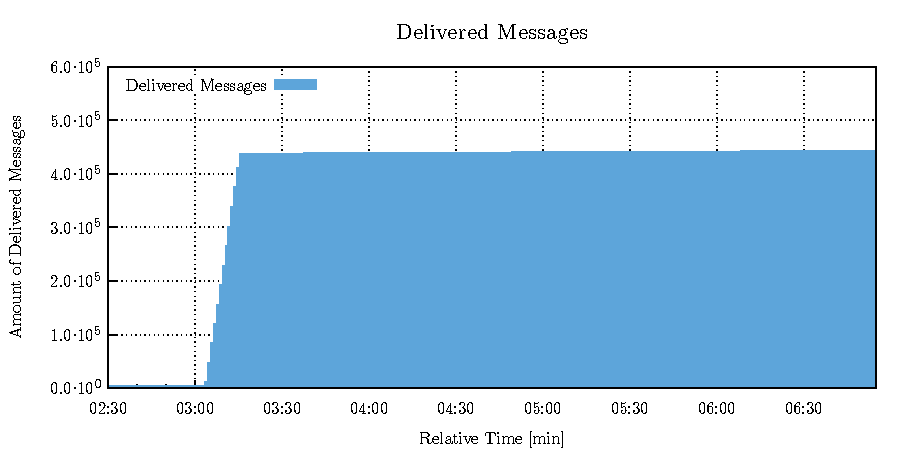
\includegraphics[width=\linewidth]{obrazky-figures/charts/shutdown_10-redundant-agent-delivered.pdf}}
	\end{minipage}
  \begin{minipage}{0.49\linewidth}
		\subfloat[60 seconds shutdown\label{fig:shutdown_60-redundant-agent-delivered}]{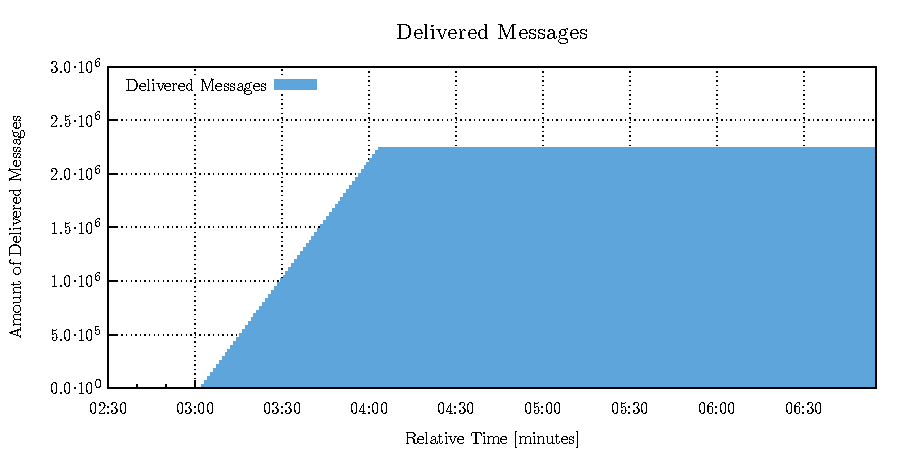
\includegraphics[width=\linewidth]{obrazky-figures/charts/shutdown_60-redundant-agent-delivered.pdf}}
	\end{minipage}
	\begin{minipage}{0.49\linewidth}
		\subfloat[120 seconds shutdown\label{fig:shutdown_120-redundant-agent-delivered}]{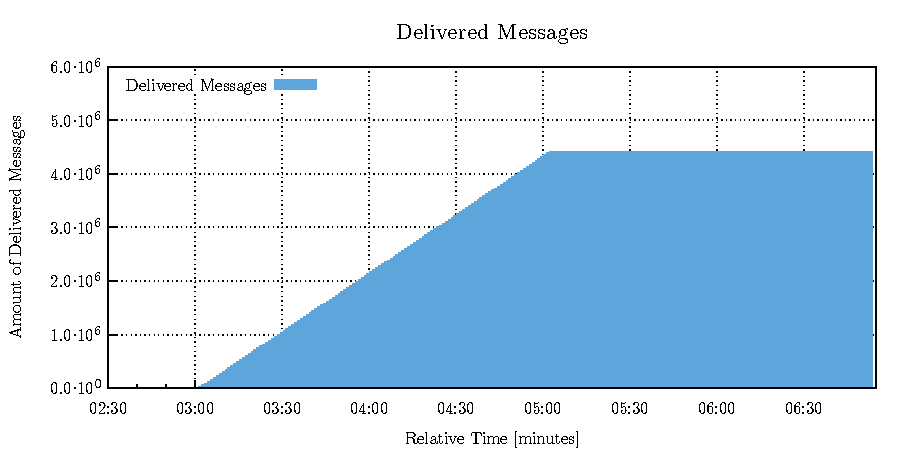
\includegraphics[width=\linewidth]{obrazky-figures/charts/shutdown_120-redundant-agent-delivered.pdf}}
	\end{minipage}
	\caption[Collected data about the delivered messages for the redundant router node during the Agent actions execution.]{Collected data about the delivered messages for the redundant router node during the Agent actions execution.}\label{fig:routerLink-latency}
\end{figure}



%\chapter{RelaxNG Schéma konfiguračního souboru} % Scheme of RelaxNG configuration file

%\chapter{Plakát} % poster
